\documentclass[11pt,a4paper]{article}
\usepackage{amsmath,amssymb,graphicx,booktabs,float,geometry,hyperref}
\usepackage[labelfont=bf]{caption}
\geometry{margin=25mm}
% drafting convenience: placeholder if a figure asset is missing
\let\origincludegraphics\includegraphics
\renewcommand{\includegraphics}[2][]{%
  \IfFileExists{#2}{\origincludegraphics[#1]{#2}}%
  {\fbox{\parbox[c][2.5cm][c]{0.75\linewidth}{\centering\ttfamily\small [missing figure asset]}}}}
\renewcommand{\thetable}{S\arabic{table}}
\renewcommand{\thefigure}{S\arabic{figure}}
\title{Electronic Supplementary Material:\\ Support Flow Tensor Field for Fast Build-Orientation Candidate Generation}
\date{}
\begin{document}
\maketitle

\section*{Supplementary Tables}

\begin{table}[H]
\footnotesize
\centering
\caption{Computation time of the four implementations for the $35$ meshes of the five groups.
$t_{\mathrm{CPU}}$ and $t_{\mathrm{CUDA}}$ are the TOMO\_CPU/TOMO\_CUDA $1^\circ$ exhaustive sweep ($\theta_c=60^\circ$) DLL times respectively,
$t_{\mathrm{py}}$ is the Python SFTF candidate evaluation, and $t_{\mathrm{C++}}$ is the SFTF\_C++ pure computation time.
hit is the number of valid face-to-face supports of the Python SFTF top direction.
The speed columns are $t_{\mathrm{CPU}}/t_{\mathrm{py}}$ and $t_{\mathrm{CPU}}/t_{\mathrm{C++}}$ respectively.
The swapped-in E-group meshes (E2, E3, E4, E9) were measured in a later session; their four rows are internally consistent but not directly comparable with the timings of the other rows.}
\label{stab:fivegroup-timing}
\resizebox{\textwidth}{!}{%
\begin{tabular}{llrrrrrrrr}
\toprule
ID & Shape & Faces & hit & $t_{\mathrm{CPU}}$(s) & $t_{\mathrm{CUDA}}$(s) & $t_{\mathrm{py}}$(s) & $t_{\mathrm{C++}}$(ms) & CPU/py & CPU/C++\\
\midrule
\multicolumn{10}{l}{\textit{A: basic shapes}}\\
A1 & cube        & 12     & 0   & 49.64 & 11.45 & 0.13 & 4.1    & $382\times$ & $12{,}108\times$\\
A2 & sphere      & 2{,}976  & 0   & 40.22 & 13.82 & 0.74 & 23.9   & $54\times$  & $1{,}683\times$\\
A3 & cylinder    & 192    & 0   & 39.64 & 22.96 & 0.17 & 1.3    & $233\times$ & $30{,}494\times$\\
A4 & cone        & 96     & 0   & 40.51 & 14.99 & 0.12 & 0.8    & $338\times$ & $50{,}641\times$\\
A5 & torus       & 2{,}304  & 184 & 43.72 & 13.57 & 0.45 & 14.2   & $97\times$  & $3{,}079\times$\\
\midrule
\multicolumn{10}{l}{\textit{B: simple parts}}\\
B1 & u\_bracket   & 28     & 2   & 40.34 & 13.91 & 0.15 & 3.9    & $269\times$ & $10{,}344\times$\\
B2 & hook        & 1{,}560  & 235 & 41.48 & 12.51 & 0.58 & 15.8   & $72\times$  & $2{,}626\times$\\
B3 & c\_clamp     & 28     & 1   & 44.82 & 17.43 & 0.17 & 0.8    & $264\times$ & $56{,}027\times$\\
B4 & pipe\_elbow  & 2{,}400  & 222 & 46.99 & 13.39 & 0.81 & 25.3   & $58\times$  & $1{,}857\times$\\
B5 & hollow\_box  & 24     & 4   & 38.63 & 17.47 & 0.21 & 0.9    & $184\times$ & $42{,}921\times$\\
\midrule
\multicolumn{10}{l}{\textit{C: organic benchmarks}}\\
C1 & \emph{Bunny 69k}       & 69{,}662 & 81  & 47.46 & 52.55 & 1.69 & 247.7 & $28\times$ & $192\times$\\
C2 & \emph{Manikin 13k}     & 13{,}672 & 134 & 37.85 & 30.44 & 1.02 & 44.3  & $37\times$ & $854\times$\\
C3 & \emph{Dragon 100k}      & 99{,}999 & 970 & 73.81 & 94.23 & 3.17 & 323.3 & $23\times$ & $228\times$\\
C4 & \emph{Happy 50k}       & 49{,}944 & 240 & 47.15 & 51.71 & 1.50 & 130.1 & $31\times$ & $363\times$\\
C5 & \emph{Lucy 50k}        & 49{,}999 & 542 & 51.15 & 71.73 & 1.87 & 172.5 & $27\times$ & $297\times$\\
\midrule
\multicolumn{10}{l}{\textit{D: Thingi10K set 1}}\\
D1  & 37009 & 23{,}909 & 57  & 51.46 & 144.10 & 1.37 & 114.5 & $38\times$ & $449\times$\\
D2  & 37010 & 13{,}247 & 35  & 45.58 & 148.94 & 1.24 & 63.5  & $37\times$ & $718\times$\\
D3  & 37011 & 17{,}288 & 82  & 52.65 & 59.75  & 1.15 & 89.2  & $46\times$ & $590\times$\\
D4  & 37091 & 256    & 42  & 46.38 & 21.23  & 0.36 & 5.2   & $129\times$ & $8{,}920\times$\\
D5  & 37095 & 468    & 65  & 38.19 & 39.54  & 0.49 & 6.2   & $78\times$ & $6{,}160\times$\\
D6  & 37111 & 88{,}106 & 386 & 99.34 & 212.38 & 3.42 & 465.4 & $29\times$ & $213\times$\\
D7  & 37137 & 64{,}078 & 434 & 73.92 & 233.45 & 2.90 & 305.5 & $25\times$ & $242\times$\\
D8  & 37402 & 8{,}322  & 119 & 40.32 & 73.76  & 2.43 & 49.7  & $17\times$ & $811\times$\\
D9  & 37415 & 13{,}340 & 77  & 44.51 & 126.27 & 2.96 & 65.4  & $15\times$ & $681\times$\\
D10 & 37416 & 12{,}036 & 66  & 43.45 & 64.44  & 3.39 & 80.4  & $13\times$ & $540\times$\\
\midrule
\multicolumn{10}{l}{\textit{E: Thingi10K set 2, large meshes}}\\
E1  & 39507 & 969{,}520   & 562   & 973.29 & 1041.71 & 16.92 & 4387.6 & $58\times$ & $222\times$\\
E2  & 790253 & 1{,}039{,}452 & 2{,}296 & 2572.14 & 4283.63 & 21.16 & 4886.7 & $122\times$ & $526\times$\\
E3  & 931902 & 1{,}050{,}398 & 233   & 2051.48 & 20037.24 & 23.93 & 6888.7 & $86\times$ & $298\times$\\
E4  & 439142 & 1{,}038{,}714 & 357   & 2431.31 & 12392.05 & 22.58 & 5589.8 & $108\times$ & $435\times$\\
E5  & 55280 & 900{,}490   & 1{,}072 & 939.61 & 1102.83 & 16.78 & 3957.9 & $56\times$ & $237\times$\\
E6  & 59197 & 786{,}432   & 699   & 776.49 & 826.30  & 17.50 & 4119.5 & $44\times$ & $188\times$\\
E7  & 61384 & 516{,}608   & 1{,}766 & 521.54 & 642.22  & 12.85 & 2065.0 & $41\times$ & $253\times$\\
E8  & 64445 & 514{,}938   & 1{,}594 & 125.46 & 211.96  & 15.05 & 2208.0 & $8.3\times$ & $57\times$\\
E9  & 82675 & 916{,}548   & 1{,}005 & 2843.64 & 2083.63 & 23.12 & 7272.6 & $123\times$ & $391\times$\\
E10 & 65942 & 754{,}688   & 1{,}175 & 765.24 & 830.14  & 22.11 & 3201.6 & $35\times$ & $239\times$\\
\bottomrule
\end{tabular}
}
\end{table}

\begin{table}[H]
\centering
\caption{Cost decomposition of the SFTF top direction of representative meshes.
Convex basic shapes (cube, sphere, cone) are pure build-plate support with hit$=0$, $R=P=0$,
and the rest show face-to-face self-support ($P$) and build-plate support ($B$) together.}
\label{stab:fivegroup-structure}
\begin{tabular}{llrrrr}
\toprule
ID & Shape & hit & $R$ & $P$ & $B$\\
\midrule
A1  & cube     & 0   & 0       & 0        & 401.5\\
A2  & sphere   & 0   & 0       & 0        & 136.6\\
A4  & cone     & 0   & 0       & 0        & 179.8\\
A5  & torus    & 184 & 15.9    & 40.3     & 209.1\\
B2  & hook     & 235 & 19.9    & 55.4     & 128.7\\
C1  & \emph{Bunny 69k}    & 81  & 1.4     & 25.2     & 176.3\\
C3  & \emph{Dragon 100k}   & 970 & 109.4   & 267.6    & 417.5\\
D6  & 37111    & 386 & 227.9   & 932.8    & 1{,}613\\
D10 & 37416    & 66  & 26.3    & 196.4    & 1{,}111\\
\bottomrule
\end{tabular}
\end{table}

\begin{table}[H]
\footnotesize
\centering
\caption{TOMO\_CPU global minimum $v_{ss}$ by critical angle on the int16-corrected grids (representative meshes; $60^\circ$ from the $1^\circ$ grid, other angles from the $3^\circ$ grid).
The support volume decreases monotonically as $\theta_c$ increases, and at $\theta_c{=}90^\circ$ almost all faces are self-supporting so $v_{ss}$ is $0$.
Before the accumulator fix a $16$-bit overflow made these minima appear as large negative numbers at high $\theta_c$; the corrected values are non-negative throughout.}
\label{stab:critangle}
\begin{tabular}{llrrrrr}
\toprule
ID & Mesh & $\theta_c{=}0^\circ$ & $30^\circ$ & $45^\circ$ & $60^\circ$ & $90^\circ$\\
\midrule
A1 & cube & 1{,}769 & 1{,}769 & 0 & 0 & 0\\
B2 & hook & 1{,}557 & 645 & 273 & 120 & 0\\
C1 & \emph{Bunny 69k} & 51{,}083 & 24{,}460 & 14{,}442 & 4{,}440 & 0\\
C3 & \emph{Dragon 100k} & 223{,}214 & 111{,}032 & 78{,}935 & 28{,}107 & 0\\
D1 & 37009 & 67{,}646 & 4{,}618 & 1{,}520 & 277 & 0\\
D6 & 37111 & 105{,}094 & 53{,}508 & 31{,}326 & 6{,}638 & 0\\
E1 & 39507 & 20{,}635 & 4{,}214 & 2{,}716 & 442 & 0\\
E7 & 61384 & 89{,}728 & 11{,}188 & 6{,}426 & 987 & 0\\
\bottomrule
\end{tabular}
\end{table}

\begin{table}[H]
\centering
\caption{Oracle (best within candidate pool) ratio by the number of coarse directions. Meshes other than \emph{Happy 50k}
already include a near-optimal direction at $512$.}
\label{stab:sampling}
\begin{tabular}{rrrrrr}
\toprule
\# coarse directions & \emph{Bunny 69k} & \emph{Manikin 13k} & \emph{Dragon 100k} & \emph{Happy 50k} & \emph{Lucy 50k}\\
\midrule
512  & 1.46 & 1.13 & 1.29 & 4.35 & 1.02\\
1024 & 1.50 & 1.11 & 1.33 & 3.94 & 1.02\\
2048 & 1.61 & 1.06 & 1.28 & \textbf{1.91} & 1.04\\
4096 & 1.62 & 1.13 & 1.27 & 1.91 & 1.30\\
\bottomrule
\end{tabular}
\end{table}

\begin{table}[H]
\centering
\caption{Best-of-3 ratio of the objective-function ablation on the corrected grids (lower is better).
The proposed objective $J=R+P+B$ and the old objective including nuclear/$\sigma_1$ are nearly identical per mesh (they differ only on \emph{Dragon 100k}).}
\label{stab:ablation}
\resizebox{\textwidth}{!}{%
\begin{tabular}{lrrrrrr}
\toprule
Ranking variant & \emph{Bunny 69k} & \emph{Manikin 13k} & \emph{Dragon 100k} & \emph{Happy 50k} & \emph{Lucy 50k} & Average\\
\midrule
$T$ (rank tuned, in-sample) & 1.18 & 1.88 & 1.28 & 2.18 & 1.20 & 1.55\\
$J=R+P+B$ (proposed)            & 1.38 & 5.02 & 1.40 & 2.08 & 1.20 & 2.22\\
$R{+}P{+}B{+}0.05S{+}0.05\sigma_1$ (old objective) & 1.38 & 5.02 & 1.46 & 2.08 & 1.20 & 2.23\\
$B$ alone                     & 1.43 & 2.65 & 1.40 & 2.56 & 1.20 & 1.85\\
$0.05S+0.05\sigma_1$ (tensor alone) & 3.16 & 7.56 & 5.16 & 2.15 & 2.66 & 4.14\\
$P$ alone                     & 3.16 & 6.87 & 4.91 & 2.34 & 3.68 & 4.19\\
\bottomrule
\end{tabular}
}
\end{table}

\begin{table}[H]
\centering
\caption{Best-of-3 ratio when sorting candidates by $J=R+P+B$ and the unified term $\tilde R=R+B$ (lower is better).
On the average excluding \emph{Happy 50k} (a narrow-basin hard case under the ranking-only point metric, resolved by local
verification in the main text), $\tilde R$ outperforms $J$.}
\label{stab:unified-b3}
\begin{tabular}{lrr}
\toprule
Mesh & $J=R{+}P{+}B$ & $\tilde R=R{+}B$\\
\midrule
\emph{Bunny 69k}   & \textbf{1.38} & 1.43\\
\emph{Manikin 13k} & 5.02 & \textbf{3.06}\\
\emph{Dragon 100k}  & 1.40 & \textbf{1.20}\\
\emph{Lucy 50k}    & 1.20 & 1.20\\
\midrule
Average (excl.\ \emph{Happy 50k}) & 2.25 & \textbf{1.72}\\
\bottomrule
\end{tabular}
\end{table}



\begin{table}[H]
\centering
\caption{Budget-matched local TOMO controls at the per-mesh SFTF top-$20$ grid-cell budget (five organic stored meshes).
The uniform-axis control matches SFTF in the mean and is better in the worst case; the warm-start value on these meshes is therefore not the window placement.}
\label{stab:budget-matched-baseline}
\small
\begin{tabular}{lrrrrr}
\toprule
Policy & Mean & Median & Max & Budget & $\le 2.0$\\
\midrule
SFTF top-$20$ local & 1.14 & 1.00 & 1.66 & 3.40\% & 5/5\\
Uniform-axis matched & \textbf{1.08} & 1.07 & \textbf{1.17} & 3.38\% & 5/5\\
Random matched (median) & 1.36 & 1.19 & 1.86 & 3.38\% & 5/5\\
\bottomrule
\end{tabular}
\end{table}

\begin{table}[H]
\centering
\caption{Adaptive Verification Escalation (AVE) from top-$10$ local TOMO verification on the five organic stored meshes.
On the corrected grids the base top-$10$ policy already keeps all five below ratio $2.0$, so the escalation only trims the mean.}
\label{stab:ave-organic}
\small
\begin{tabular}{lrrrrr}
\toprule
Policy & Expanded & Mean & Max & Budget & $\le 2.0$\\
\midrule
Top-$10$ local & 0/5 & 1.18 & 1.84 & 2.03\% & 5/5\\
AVE & 3/5 & \textbf{1.14} & \textbf{1.66} & 9.99\% & 5/5\\
\bottomrule
\end{tabular}
\end{table}

\begin{table}[H]
\centering
\small
\caption{Spearman rank correlation between features and TOMO $v_{ss}$ over the entire candidate pool.
The larger the positive value, the more valid the feature is as a cost.}
\label{stab:feature-corr}
\begin{tabular}{lrrrrrr}
\toprule
Feature & \emph{Bunny 69k} & \emph{Manikin 13k} & \emph{Dragon 100k} & \emph{Happy 50k} & \emph{Lucy 50k} & Average\\
\midrule
$J=R{+}P{+}B$         & 0.37 & 0.35 & 0.80 & 0.33 & 0.68 & 0.51\\
$R$ (Rayleigh)        & 0.36 & $-0.35$ & $-0.56$ & 0.13 & 0.16 & $-0.05$\\
$P$ (pair flow)       & $-0.09$ & $-0.41$ & $-0.71$ & 0.10 & $-0.67$ & $-0.36$\\
$B$ (build-plate)     & \textbf{0.42} & \textbf{0.74} & \textbf{0.84} & \textbf{0.23} & \textbf{0.72} & \textbf{0.59}\\
$H$ (hit count)       & 0.24 & $-0.58$ & $-0.72$ & 0.13 & $-0.82$ & $-0.35$\\
$S$ (nuclear)         & $-0.07$ & $-0.39$ & $-0.69$ & 0.08 & $-0.29$ & $-0.27$\\
$\sigma_1$            & $-0.09$ & $-0.36$ & $-0.65$ & 0.05 & 0.07 & $-0.20$\\
\bottomrule
\end{tabular}
\end{table}

\begin{table}[H]
\centering
\caption{LOMO cross-validation best-of-3 ratio of rank tuning (lower is better).
The in-sample column is the calibration-set fit value; the oracle is the best direction existing within the candidate pool.}
\label{stab:lomo-cv}
\begin{tabular}{lrrrr}
\toprule
Mesh & oracle & untuned $J$ & in-sample (reported) & LOMO\\
\midrule
\emph{Bunny 69k}    & 1.02 & 1.38 & 1.21 & 1.21\\
\emph{Manikin 13k}  & 1.17 & 5.02 & 2.87 & 3.02\\
\emph{Dragon 100k}   & 1.03 & 1.40 & 1.41 & 1.41\\
\emph{Lucy 50k}     & 1.01 & 1.20 & 1.10 & 1.20\\
\midrule
Average     & 1.06 & 2.25 & \textbf{1.64} & \textbf{1.71}\\
\bottomrule
\end{tabular}
\end{table}

\begin{table}[H]
\centering
\caption{Unified comparison of existing methods and SFTF (best-of-3 signed $v_{ss}$ ratio, lower is better).
SFTF-tuned is the five-mesh LOMO estimate for rank-only candidate ordering.}
\label{stab:unified}
\begin{tabular}{lrrrrr}
\toprule
Mesh & PCA & Support Tensor & SFTF untuned & SFTF tuned (LOMO) & oracle\\
\midrule
\emph{Bunny 69k}    & 1.55 & 2.11 & 1.38 & 1.21 & 1.02\\
\emph{Manikin 13k}  & 2.90 & 2.39 & 5.02 & 3.02 & 1.17\\
\emph{Dragon 100k}   & 2.10 & 1.58 & 1.40 & 1.41 & 1.03\\
\emph{Lucy 50k}     & 1.26 & 3.76 & 1.20 & 1.20 & 1.01\\
\midrule
Average     & 1.95 & 2.46 & 2.25 & \textbf{1.71} & 1.06\\
\bottomrule
\end{tabular}
\end{table}

\begin{table}[H]
\footnotesize
\centering
\caption{Group-wise average execution time and speed ratio.
The C++ SFTF average is in ms, and the TOMO and Python SFTF averages are in seconds.}
\label{stab:fivegroup-impl}
\begin{tabular}{lrrrrrr}
\toprule
& \multicolumn{2}{c}{TOMO} & \multicolumn{2}{c}{SFTF} & \multicolumn{2}{c}{comparison}\\
\cmidrule(lr){2-3}\cmidrule(lr){4-5}\cmidrule(lr){6-7}
Group & CPU (s) & CUDA (s) & py (s) & C++ (ms) & CPU/py & CPU/C++\\
\midrule
A & 42.75  & 15.36  & 0.32 & 8.9    & $54.4$--$381.9\times$   & $1{,}683$--$50{,}641\times$\\
B & 42.45  & 14.94  & 0.38 & 9.3    & $58.0$--$269.0\times$   & $1{,}857$--$56{,}027\times$\\
C & 51.48  & 60.13  & 1.85 & 183.6  & $23.3$--$36.9\times$   & $192$--$854\times$\\
D & 53.58  & 112.38 & 1.97 & 124.5  & $12.8$--$128.8\times$  & $213$--$8{,}920\times$\\
E & 1400.02 & 4345.17 & 19.20 & 4457.7 & $8.3$--$123.0\times$    & $56.8$--$526.4\times$\\
\bottomrule
\end{tabular}
\end{table}

\section*{Supplementary Figures}

\begin{figure}[H]
\centering
% The capture file is draft/pics/_5G_CA60deg_best_worst_grouped.png
% generated by re-arranging and labeling per group with scripts/render_figure6_grouped.py.

\includegraphics[width=\textwidth]{pics/_5G_CA60deg_best_worst_grouped.png}
\caption{Best/worst build-orientation Polyscope overlay arranged by group for the five groups (A--E) ($\theta_c=60^\circ$).
A label is placed atop each group, with groups A--C in the top row and groups D/E (a vertical $5$-row $2$-column layout each) in the bottom row, grouped about the page center.
Each mesh shows the original (gray), optimal orientation (blue), and worst orientation (red) side by side,
displayed in the actual print pose by rotating the stored build direction to world $+Z$.
Since SFTF candidates are invariant to $\theta_c$, the overlays of the five critical angles are identical.}
\label{sfig:five-group-best-worst}
\end{figure}

\begin{figure}[H]
\centering
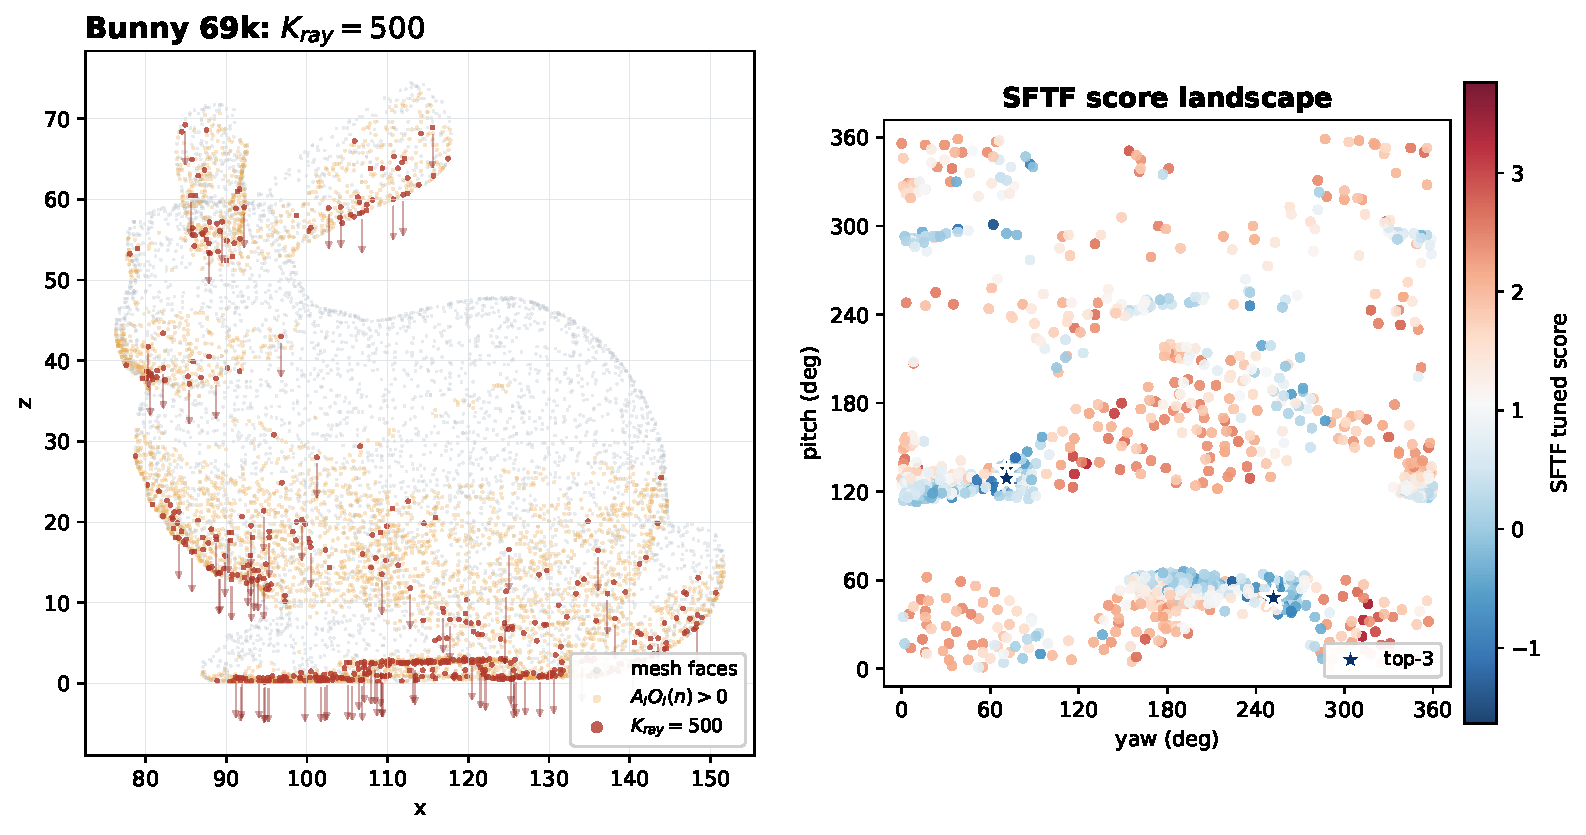
\includegraphics[width=\textwidth]{pics/Bunny69k_kray500_concept.pdf}
\caption{\emph{Bunny 69k} source-face sampling and SFTF score landscape with fixed $K_{ray}=500$.
The right panel is recomputed with the same ray budget and uses the common color scale of Supplementary Figs.~\ref{sfig:bunny-kray1394}--\ref{sfig:bunny-kray3000}.}
\label{sfig:bunny-kray500}
\end{figure}

\begin{figure}[H]
\centering
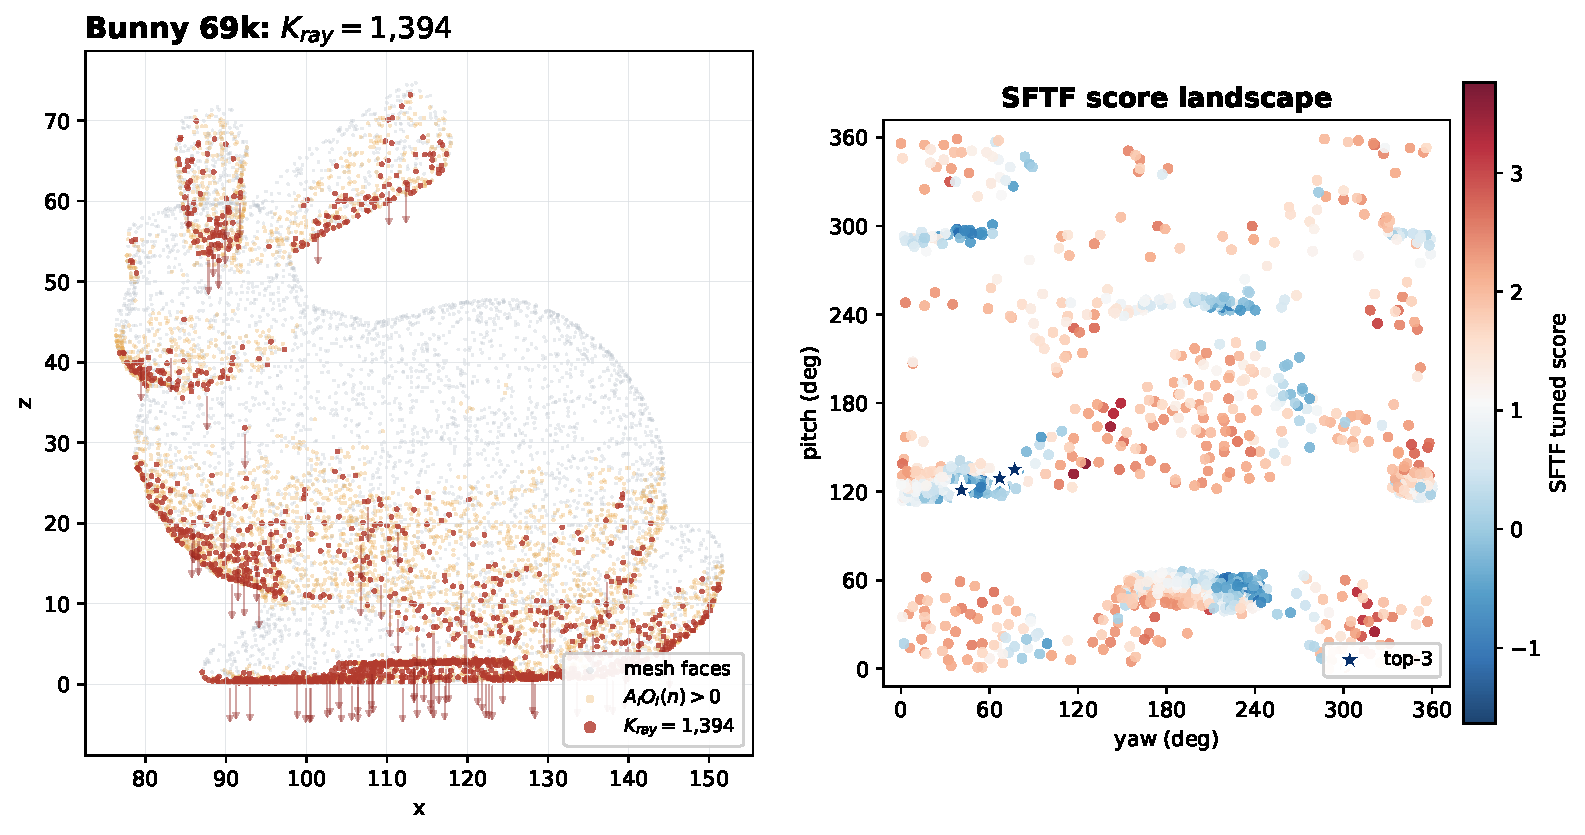
\includegraphics[width=\textwidth]{pics/Bunny69k_kray1394_concept.pdf}
\caption{\emph{Bunny 69k} source-face sampling and SFTF score landscape with the adaptive rule, $K_{ray}=\mathrm{clip}(0.02N_f,500,3000)=1{,}394$.}
\label{sfig:bunny-kray1394}
\end{figure}

\begin{figure}[H]
\centering
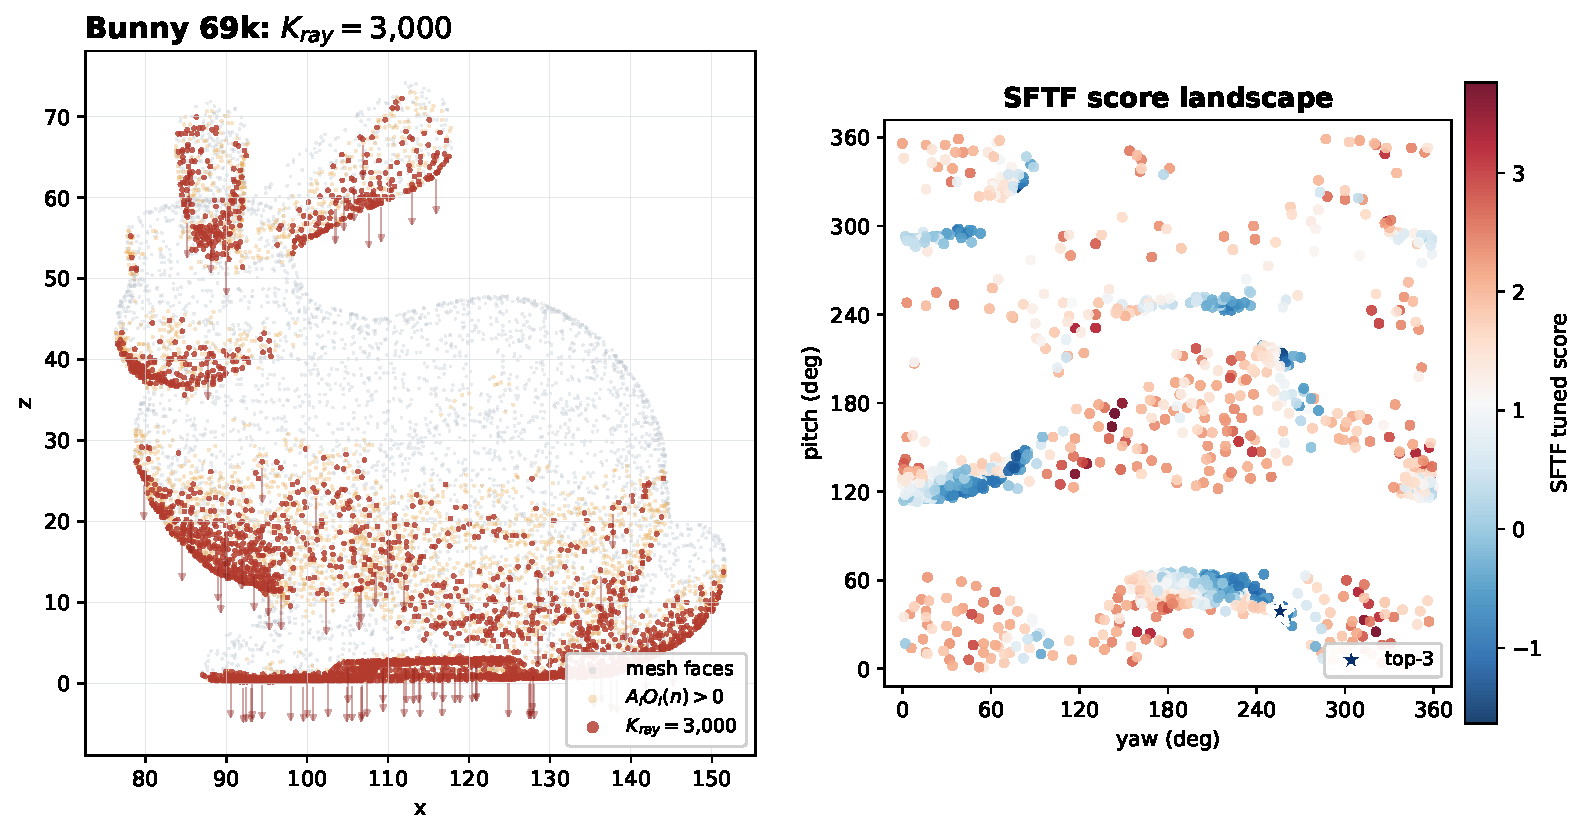
\includegraphics[width=\textwidth]{pics/Bunny69k_kray3000_concept.pdf}
\caption{\emph{Bunny 69k} source-face sampling and SFTF score landscape with fixed $K_{ray}=3000$, corresponding to the upper cap used for large meshes.}
\label{sfig:bunny-kray3000}
\end{figure}

\begin{figure}[H]
\centering
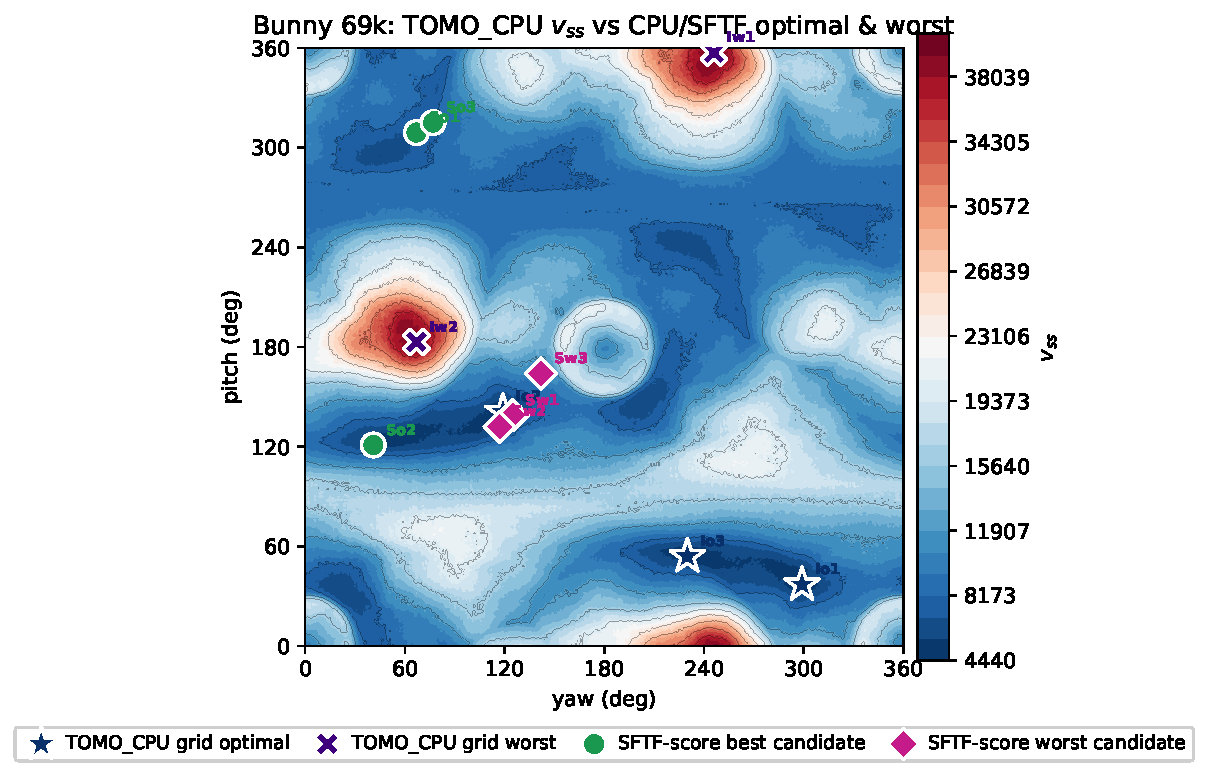
\includegraphics[width=0.78\linewidth]{pics/appendix_contour_bunny.pdf}
\caption{Comparison of CPU/SFTF optimal/worst orientations on the TOMO\_CPU $v_{ss}$ landscape of \emph{Bunny 69k} (blue is good).
The markers are 3 each of CPU/SFTF optimal/worst, with kinds following the legend below the figure.
The global optimum is $v_{ss}=4440$ (yaw$=299^\circ$, pitch$=37^\circ$; the corrected main-text comparison table),
and lies not at a single point but within a broad low-cost basin.}
\label{sfig:bunny-landscape}
\end{figure}

\begin{figure}[H]
\centering
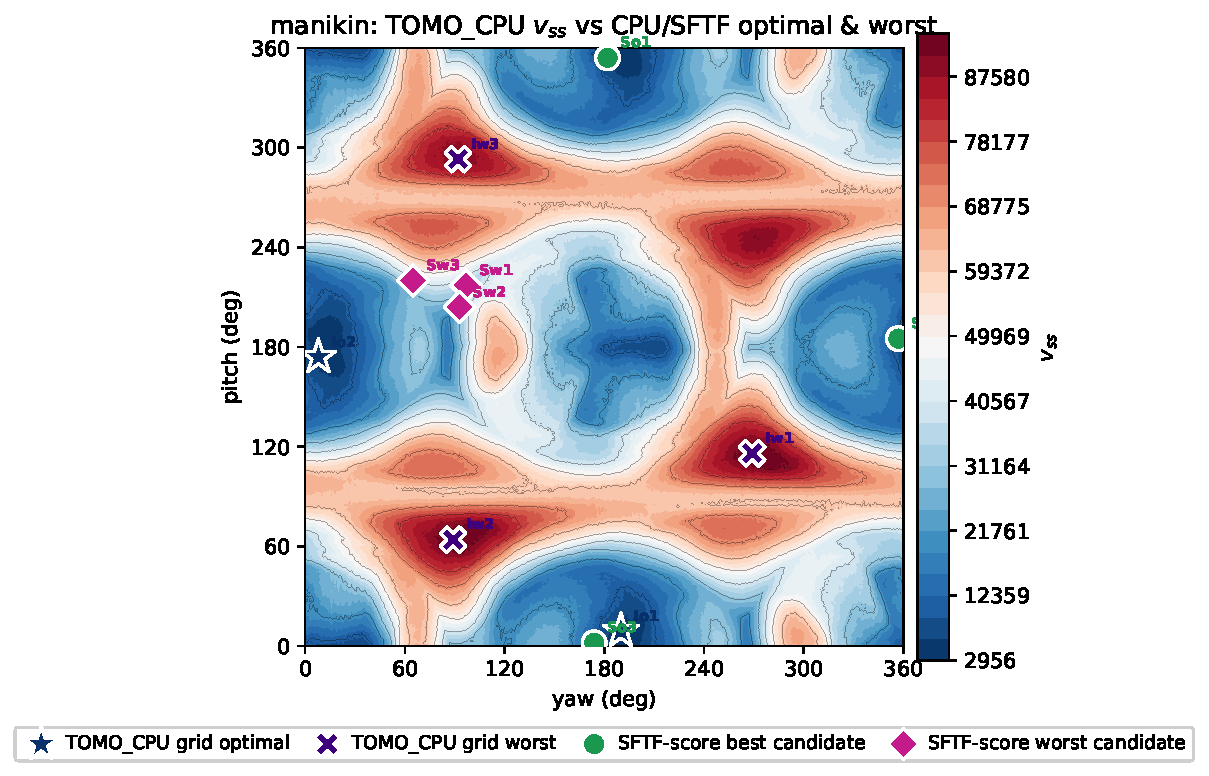
\includegraphics[width=0.78\linewidth]{pics/appendix_contour_manikin.pdf}
\caption{Comparison of CPU/SFTF optimal/worst orientations on the TOMO\_CPU $v_{ss}$ landscape of \emph{Manikin 13k} (blue is good).
The markers are 3 each of CPU/SFTF optimal/worst, with kinds following the legend below the figure.
The global optimum is $v_{ss}=2956$ (yaw$=190^\circ$, pitch$=9^\circ$), and
befitting a vertically elongated shape, the low-cost region is distributed in a narrow pitch band across the full yaw range.}
\label{sfig:manikin-landscape}
\end{figure}

\begin{figure}[H]
\centering
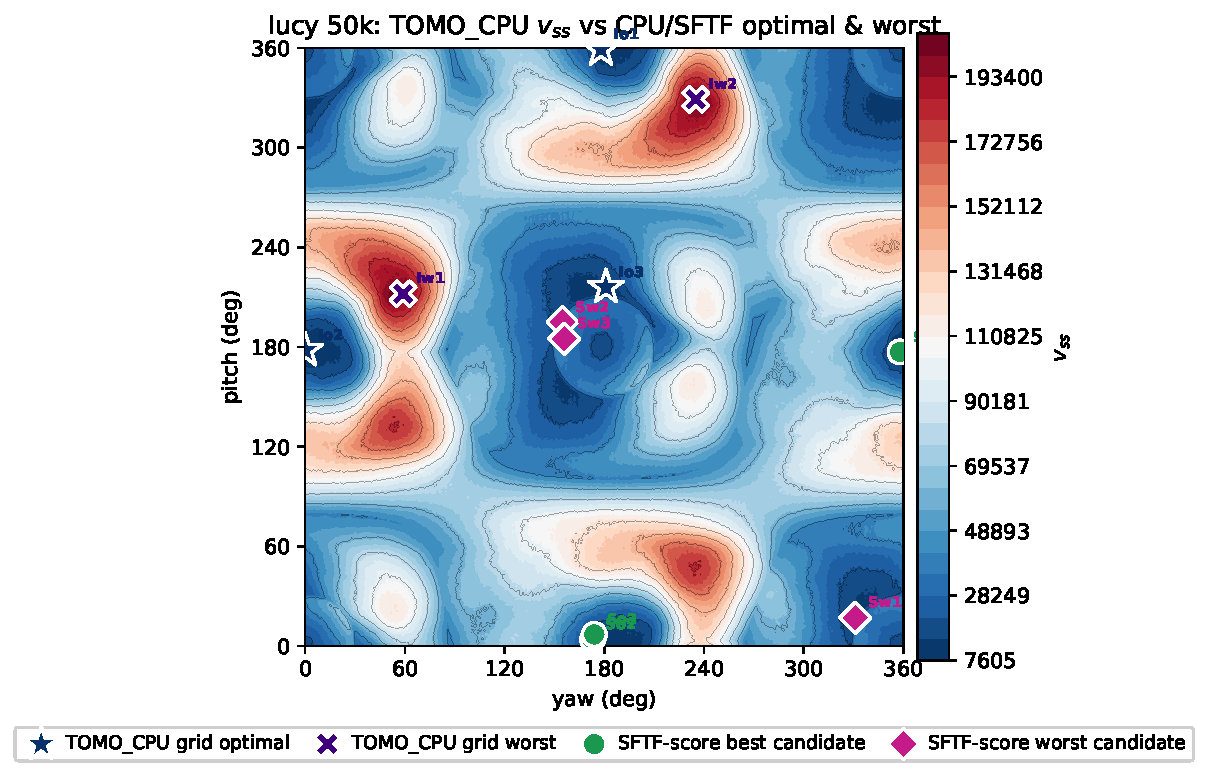
\includegraphics[width=0.78\linewidth]{pics/appendix_contour_lucy.pdf}
\caption{Comparison of CPU/SFTF optimal/worst orientations on the TOMO\_CPU $v_{ss}$ landscape of \emph{Lucy 50k} (blue is good).
The markers are 3 each of CPU/SFTF optimal/worst, with kinds following the legend below the figure.
The global optimum is $v_{ss}=7605$ (yaw$=178^\circ$, pitch$=359^\circ$), and
being located near the pitch boundary ($359^\circ$), it requires basin search that considers the yaw--pitch periodicity.}
\label{sfig:lucy-landscape}
\end{figure}


\end{document}
